\documentclass[letterpaper,11pt]{article}

% Soporte para los acentos.
\usepackage[utf8]{inputenc}
\usepackage[T1]{fontenc}
% Idioma español.
\usepackage[spanish,mexico, es-tabla]{babel}
% Soporte de símbolos adicionales (matemáticas)
\usepackage{multirow}
\usepackage{amsmath}
\usepackage{amssymb}
\usepackage{amsthm}
\usepackage{amsfonts}
\usepackage{mathtools}
\usepackage{latexsym}
\usepackage{enumerate}
\usepackage{ragged2e}
\usepackage{listings}
\usepackage{xcolor}
\usepackage{graphicx}
\usepackage{hyperref}
% Modificamos los márgenes del documento.                                       %
\usepackage[lmargin=2cm,rmargin=2cm,top=2cm,bottom=2cm]{geometry}

\definecolor{codegreen}{rgb}{0,0.6,0}
\definecolor{codegray}{rgb}{0.5,0.5,0.5}
\definecolor{codepurple}{rgb}{0.58,0,0.82}
\definecolor{backcolour}{rgb}{0.95,0.95,0.92}

\lstdefinestyle{mystyle}{
    backgroundcolor=\color{backcolour},   
    commentstyle=\color{codegreen},
    keywordstyle=\color{magenta},
    numberstyle=\tiny\color{codegray},
    stringstyle=\color{codepurple},
    basicstyle=\ttfamily\footnotesize,
    breakatwhitespace=false,         
    breaklines=true,                 
    captionpos=b,                    
    keepspaces=true,                 
    numbers=left,                    
    numbersep=5pt,                  
    showspaces=false,                
    showstringspaces=false,
    showtabs=false,                  
    tabsize=2
}

\lstset{style=mystyle}

\title{Facultad de Ciencias, UNAM \\ Redes Neuronales \\ Tarea 2}
\author{Rubí Rojas Tania Michelle}
\date{13 de abril de 202}

\begin{document}
\maketitle

\begin{enumerate}
    % Ejercicio 1.
    \item Usando \textit{sklearn.datasets.make moons} genera un conjunto de 
    datos de la siguiente forma:
    \begin{verbatim}
        In [1]: C1, C2 = moons(random state=123, n samples=200, noise=0.1)
    \end{verbatim}

    \begin{lstlisting}[language=Python]
        from sklearn.datasets import make_moons
        import matplotlib.pyplot as plt

        # Generamos un conjunto de datos.
        C1, C2 = make_moons(random_state = 123, n_samples=200, noise=0.1)
        plt.scatter(C1[:,0], C1[:,1], c=C2); plt.show()
    \end{lstlisting}

    \begin{figure}[h]
        \centering
        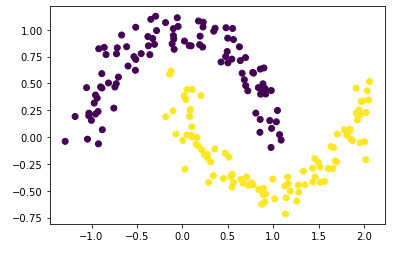
\includegraphics[width=0.5\textwidth]{./imagenes/datos.png}
    \end{figure}            

    \begin{enumerate}
        % Ejercicio 1.a
        \item Implementa la regresión logística usando el descenso gradiente 
        para clasificar $C_1$ y $C_2$. 

        % Ejercicio 1.b
        \item ¿Qué transformación de los datos ocupaste para poder hacer la
        correcta clasificación?
    \end{enumerate}

    % Ejercicio 2.
    \item Calcula la derivada de la tangente hiperbólica $\tanh$.
    
    \textsc{Solución:}
    \begin{align*}
        \frac{d}{dx} \tanh (x) 
        &= \frac{d}{dx} \left(\frac{\sinh (x)}{\cosh (x)}\right)
        && \text{definición de $\tanh (x)$} \\
        &= \frac{(\sinh' (x) \cdot \cosh (x)) - (\cosh' (x) \cdot \sinh (x))}
                {\cosh^2 (x)}
        && \text{derivative quotient rule} \\ 
        &= \frac{(\cosh (x) \cdot \cosh (x)) - (\sinh (x) \cdot \sinh (x))}
                {\cosh^2 (x)}
        && \text{$\sinh' (x) = \cosh (x)$ y $\cosh' (x) = \sinh (x)$} \\ 
        &= \frac{\cosh^2 (x) - \sinh^2 (x)}{\cosh^2 (x)}
        && \text{aritmética} \\ 
        &= \frac{1}{\cosh^2 (x)}
        && \text{$\cosh^2 (x) - \sinh^2 (x) = 1$} \\ 
        &= sech^2 (x)
        && \text{$\frac{1}{\cosh^2} = sech^2 (x)$}
    \end{align*}

    % Ejercicio 3.
    \item Usando el perceptrón multicapa visto en clase, clasifica a $C_1$ y 
    $C_2$. ¿Qué parámetros ocupaste?

    % Ejercicio 4.
    \item Con la red neuronal, vista en clase, que hace la clasificación 
    multiclase usando la función \textit{softmax}, realiza los siguiente 
    ejercicios:
    \begin{enumerate}
        % Ejercicio 4.a
        \item Encuentra la mejor arquitectura para el conjunto de Iris. 
        Justifica tu respuesta de por qué es la mejor.

        % Ejercicio 4.b
        \item Usa las funciones $\tan h$ y $\gamma$ en la capa intermedia. ¿Cuál
        funciona mejor?

        % Ejercicio 4.c
        \item Clasifica los siguientes estímulos y reporta a qué clase pertenece
        cada uno:
        \begin{itemize}
            \item $5.97 \; 4.20 \; 1.23 \; 0.25$
            \item $6.80 \; 5.00 \; 1.25 \; 1.20$
            \item $12.50 \; 9.20 \; 40.32 \; 21.55$
        \end{itemize}

        % Ejercicio 4.d
        \item ¿Te parecen correctas todas las clasificaciones? En caso de que 
        alguna no, ¿por qué? ¿cómo corregirías este error?
    \end{enumerate}

    % Ejercicio 5.
    \item ¿Qué es y cómo funciona la función de activación \textit{Radial Basis
    Function (RBF)}?

    \textsc{Solución:} Una \textit{función de base radial} $\phi(x)$ es una 
    función que calcula la distancia euclideana de un vector de entrada $x$
    respecto de un centro $c$, de tal manera que resulta la siguiente función:
    \begin{equation*}
        f(x) = (\| x - c_i\|)
    \end{equation*}

    A cada neurona de la capa de entrada le corresponde una función de base 
    radial $\Phi (x)$ y un peso de salida $w_i$. El patrón de salida ingresa a
    una neurona de salida que suma las entradas y da como resultado una salida.
    La función de una red $RBF$ final resulta:
    \begin{equation*}
        F(x) = \sum^N_{i=1} w_{i} \Phi (\| x - c_{i} \|)
    \end{equation*} 

    Las redes $RBF$ tienen una construcción rígida de tres capas:
    \begin{figure}[ht]
        \centering
        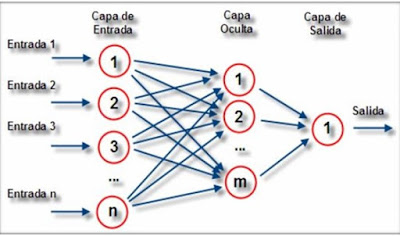
\includegraphics[width=0.4\textwidth]{./imagenes/rbf.png}
    \end{figure}  

    \begin{itemize}
        \item \textbf{Capa de Entrada}. Transmiten las señales de entrada a las 
        neuronas ocultas sin realizar procesamiento, es decir, las conexiones de 
        la capa de entrada a la capa oculta no llevan pesos asociados. 

        \item \textbf{Capa Oculta}. Realizan una transformación local y no lineal 
        de dichas señales.

        Cada elemento de procesado $i$ de la capa oculta tiene asociada una 
        función de base radial de tal manera que representa una clase o 
        categoría, donde dicha clase viene dada por $(C_i, d_i)$. $C_i$
        representa un centro de cluster (pesos asociados a cada neurona $i$) y 
        $d_i$ representa la desviación, anchura o dilatación de la función de 
        base radial asociada a dicho elemento. 

        La salida de cada elemento de la capa oculta $z_i (n)$ se calcula como 
        ls distancia que existe entre el patrón de entrada $X (n)$ al centro del 
        clouster $C_i$ ponderada inversamente por $d_i$, y aplicando después a 
        ese valor una función de base radial.
        \begin{equation*}
            z_i (n) = 
            \Phi \left(\frac{\left( \sum^p_{j=1} \left( x_j (n) - c_{ji} 
                                                 \right)^2 \right)^{\frac{1}{2}}}
                            {d_i} \right) \; \; \; \; \; \; \; \; \; 
            i \in \{1, 2, ..., m\}
        \end{equation*}

        donde $\Phi$ es una función de base radial, dentro de éstas la más 
        utilizada es la función Gaussiana 
        \begin{equation*}
            \Phi (r) = e^{\frac{-r^2}{2}}
        \end{equation*}

        \item \textbf{Capa de Salida}. Realiza una combinación de las actividades 
        de las neuronas ocultas. Tiene la responsabilidad en la red de activación 
        de patrones aplicados en la capa de entrada. 

        Cada elemento de procesado calcula su valor neto como una combinación
        lineal de las salidas de los elementos de procesado de la capa oculta.
        La función de activación y transferencia es lineal, por lo que para un 
        patrón $n$, $X(n) = (x_1 (n), x_2 (n), ..., x_p (n))$, la salida de la 
        red asociada a cada elemento $k$ de la capa de salida se obtiene de la 
        forma 
        \begin{equation*}
            y_k (n) = \sum^m_{i=1} w_{ik} z_i (n) + \mu_k \; \; \; \; \; \; \;
            k \in \{1, 2, ..., r\}
        \end{equation*}

        donde los $w_{ik}$ son los pesos asociados al elemento $k$ de la capa 
        oculta y el elemento $i$ de la capa oculta, que ponderan cada uno las 
        salidas $z_i (n)$ del elemento de procesado de la capa oculta 
        correspondiente. 

        El término $\mu_k$ es un término denominado umbral y está asociado a
        cada uno de los elementos de procesado de la capa de salida. 
    \end{itemize}

    El aprendizaje consiste en la determinación de centros, desviaciones y pesos 
    de la capa oculta a la capa de salida. Como las capas de la red realizan 
    diferentes tareas, se separaán los parámetros de la capa oculta de la capa 
    de salida para optimizar el proceso. De esta forma, los centros y las 
    desviaciones siguen un proceso guiado por una optimización en el espacio de 
    entrada, mientras que los pesos siguen una optimización sobre la base de las 
    salidas que se desean obtener. 

    Los métodos de aprendizaje más utilizados son el \textit{método híbrido} y
    el \textit{método totalmente supervisado}. 
\end{enumerate}

\textbf{Bibliografía}
\begin{itemize}
    \item \url{https://www.wikiwand.com/es/RNA_de_base_radial#/Referencias}
    \item \url{http://ele.aut.ac.ir/~abdollahi/Lec_3_NN11.pdf}
    \item \url{http://dianainteligenciaartificial.blogspot.com/2015/07/redes-de-
               neuronas-de-base-radial.html}
    \item \url{http://www.varpa.org/~mgpenedo/cursos/scx/archivospdf/Tema5-6.pdf}
\end{itemize}
\end{document}
